In diesem Grundlagenkapitel werden Erfolgschancen für Unternehmen aufgelistet, die Cloud-Dienste in ihre Geschäftsprozesse integrieren.
\\
Folgenden Ergebnisse können erreicht werden, wenn die Überwachung- und Optimierungsmaßnahmen eingeführt werden.
\begin{itemize}
      \item
            Die Möglichkeit, die individuellen Kosten verschiedener Projekte die über dieselbe Infrastruktur laufen, zu erkennen. Auf diese Weise ist es auch möglich, eine Unterscheidung zwischen Kunden, die mehr oder weniger Ressourcen verbrauchen, zu machen.
      \item
            Eine beachtliche Erhöhung der (finanziellen) Rentabilität im Unternehmen.
      \item
            Eine geringere Ungewissheit, bei der Umsetzung von cloudbasierten Systemen.
      \item
            Mehr Kontrolle auf die  Gesamtkosten des Betriebs (TCO).
            
\end{itemize}


\begin{flushleft}
      Es wird erklärt warum die Kostenoptimierung und -überwachung relevant für Unternehmen sind.
\end{flushleft}
%Basandose en "Vor- und Nachteile der Nutzung von Cloud-Diensten (mit mobilen Endgeräten) in Organisationen und deren Einfluss auf die Nachhaltigkeit"
% Debería aclarar los aspectos principales de mi BA
% En mi caso: 

%1-Cuales son los miedos, razones y oportunidades para las empresas en la NUBE?

%\subsection{Risiken und Oportunitäten der Cloud...}\label{subsec_UabsGrund2}
%Vor- und Nachteile / ?

\subsection{Ökonomie des Cloud Computing}\label{subsec_UabsGrund3}
%Was bietet die Cloud den Unternehmen?
%Economics of Cloud Computing
%https://d1.awsstatic.com/whitepapers/introduction-to-aws-cloud-economics-final.pdf
[Date last review: 00.00]
\begin{flushleft}
      {
            Cloud Economics auf Englisch, basierend auf dem On-Demand Prinzip basiert,
            gibt die Flexibilität, Rechenkapazität je nach Bedarf anzupassen.
            %entweder manuell oder automatisch
            Es entfallen große Investitionen in der Hardware, wie bei On-Premise-Systemen.
            Durch den Verzicht auf Hardware entfallen die Kosten für Reparatur, Wartung und eventuell damit verbundene Lizenzen. 
            \\
            Der Cloud-Anbieter übernimmt viele Verwaltungsaufgaben. Das führt zu einer Abnahme der nötigen Fachkraft.
            {\cite{IDC01}}


            Die Nutzung dieser Dienste ist innerhalb weniger Minuten und in unabhängiger Weise möglich 
            (IST DAMIT KLAR, DASS ICH Selbsbedienung MEINE?). }
\end{flushleft}

Grafik der Kosten On-Premise/Demand?

\subsubsection{Skalierbarkeit}
Um die Leistung aufrecht zu halten und bei Abnahme der Nachfrage diese zu reduzieren,  ist es möglich die Rechenkapazität automatisch hoch und runter zu skalieren.

Mit Auto Scaling wird sichergestellt, dass die Anzahl der Amazon Server-Instanzen während
Nachfragespitzen(IST DAS WORT VERSTÄNDLICH?) nahtlos hochskaliert werden.
% und damit Kosten minimieren.
Auf diese Weise kann weniger Zeit mit der Verwaltung von IT-Ressourcen verbracht werden und sich mehr auf wesentliche Geschäftsaktivitäten konzentrieren konzentriert werden.
\\\\
Dies war der Fall bei Walgreens in den USA.
Sie haben unter anderem 750 virtuelle Maschinen und SAP HANA auf Azure Instanzen migriert.

\begin{quote}
      „One of the key reasons for moving to Azure was so that we could take advantage of the scalability that SAP HANA is capable of„
      \\
      Dan Regalado: Vice President of Global Technology Transformation and Strategic Partnerships Walgreens Boots Alliance
            {\cite{AZU01}}
\end{quote}

\subsubsection{Flexibilität und Agilität}
In der Amazon Web Services gibt es im Allgemeinen eine Auswahl zwischen folgenden Optionen.
\begin{itemize}
      \item
            Aus verschiedenen Betriebssystemen, mit und ohne Lizenzierung.
      \item
            Zwischen den meistverbreitete Programmiersprachen unter anderem Java, C++, Go, JavaScript Python und mehr.
      \item
            Hosting von statischen Webseiten und Webanwendungen.
      \item
            Populäre relationale und nicht relationale Datenbanken.
      \item
            Vielfältige Hardware-Konfigurationen.

\end{itemize}
\begin{flushleft}
      Durch die Vielzahl der verfügbaren Optionen ist es möglich, Prototypen oder Experimente in kurzer Zeit durchzuführen.
      {\cite{IDC01}}, S. 7.
      Die neue Entwicklung kann auf dem Markt mit echtem Kundenfeedback getestet werden.
      \\
      %Je nach ihrer Akzeptanz im Markt ist es möglich, sinnvolle Entscheidungen zu treffen.
      Wenn die Neuentwicklung nicht erfolgreich war, fallen keine Kosten an.
      Da die verwendete Dienste vollständig stillgelegt werden können.
\end{flushleft}
{\cite{AMZ03, AMZ04}}

\subsubsection{Selbstbedienung}
Mit geringem Aufwand ist es möglich, Cloud-Dienste eigenständig zu nutzen. Dies ist allerdings ein zweischneidiges Schwert.
MACHT DAS SINN?
Zum einen werden keine Vermittler(ICH MEINE HIER AUTO SERVICE. IST ES KLAR?) benötigt, um die gewünschten Dienste einzurichten. Andererseits besteht die Gefahr, dass hohe Kosten entstehen.

TODO: LOOK FOR A USE CASE WHEREE THIS HAPPEND

\subsubsection{Keine Vorabkosten}
%https://aws.amazon.com/de/ec2/pricing/
Amazon Web Services bietet ein Pay-as-you-go-Modell für Ressourcen in On-Demand Zahlungsmodell.
Diese werden nach einer bestimmten Einheit wie GB/Stunde für Speichereinheiten berechnet.
\\\\
Im Fall von Server-Instanzen wird es ein Stundensatz auf der Grundlage \newline der Servereigenschaften festgelegt.

Hier einige Beispiele von EC2-Instanzen in On-Demand Zahlungsmodell.

\begin{center}
      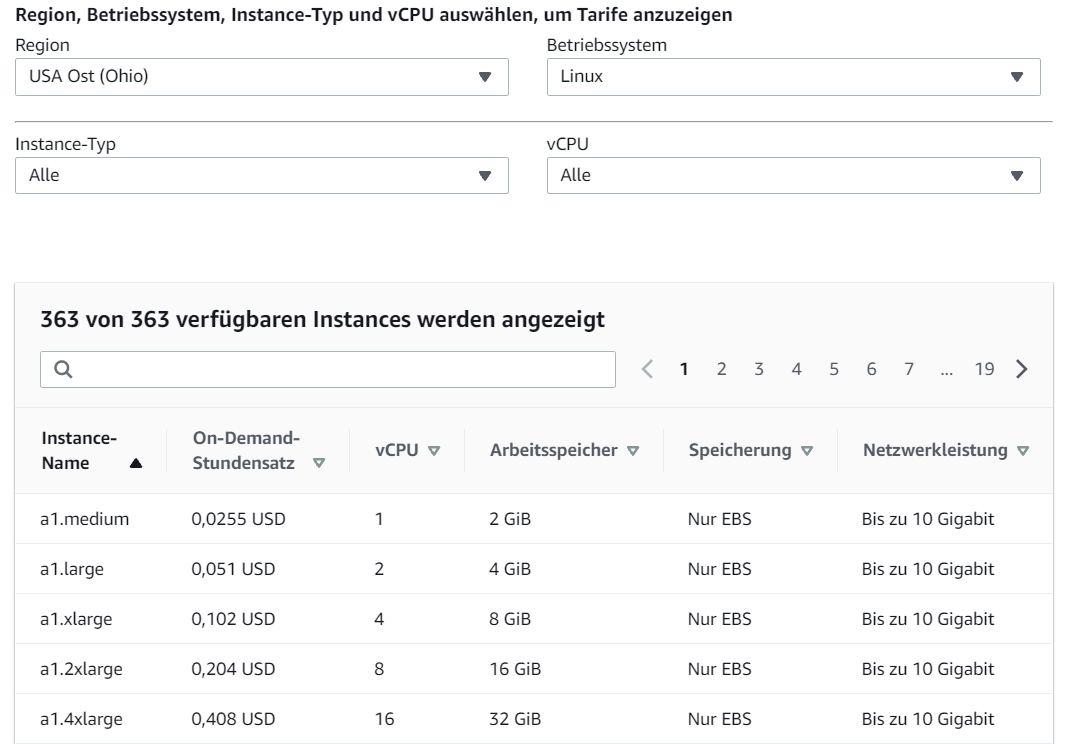
\includegraphics[scale=0.4]{sources/On-Demand-Pläne für Amazon EC2}\label{fig:OnDemand_Preise}\\
      \textbf{Abbildung \autoref{fig:OnDemand_Preise}:} On-Demand Preise für Amazon EC2
      \footnote{Vgl. u.a.\cite{AMZ01}}
\end{center}
Dies ist jedoch nicht das einzige Zahlungsmodell für Server-Instanzen bei AWS.
\\
 Mehr dazu in Kapitel 4 Zahlungsmodelle.
\begin{comment}
Advantages of Cloud Technology
As the technology has matured over the last decade, companies are moving to the
cloud to lower costs, reduce complexity, and increase flexibility. The cloud
provides scalable and powerful compute solutions, low-cost, reliable storage, and addition, cloud technologies can be used to deploy solutions quickly and cost effectively around the world and on any device.
When you decouple from the data center, you’ll be able to:
x Decrease your TCO: Eliminate many of the costs related to building and
maintaining a data center or colocation deployment. Pay for only the
resources you consume.

x Reduce complexity: Reduce the need to manage infrastructure,
investigate licensing issues, or divert resources.
x Adjust capacity on the fly: Add or reduce resources, depending on
seasonal business needs, using infrastructure that is secure, reliable, and
broadly accessible.
x Reduce time to market: Design and develop new IT projects faster.
x Deploy quickly, even worldwide: Deploy applications across multiple
geographic areas.
x Increase efficiencies: Use automation to reduce or eliminate IT
management activities that waste time and resources.
x Innovate more: Spin up a new server and try out an idea. Each project
moves through the funnel more quickly because the cloud makes it faster
(and cheaper) to deploy, test, and launch new products and services.
x Spend your resources strategically: Switch to a DevOps model to free
your IT staff from operations and maintenance that can be handled by the
cloud services provider.
x Enhance security: Spend less time conducting security reviews on
infrastructure. Mature cloud providers have teams of people who focus on
security, offering best practices to ensure you’re compliant, no matter what
your industry.
\end{comment}

%\subsection{Was ist EC2? To Review}\label{subsec_UabsGrund4}
%Man kann HW und SW auswählen


% Amazon video Cloud Eco.: https://www.youtube.com/watch?v=kUNBx1MTwxw
% short explaniation https://www.youtube.com/watch?v=RI9RTbXEjLc
%3- Hard and Soft Savings https://youtu.be/Q5wSvUVPyYY?t=316
% Suche ein Buch, mit info darüber!

%\subsection{Dienste für ein Standard-Anwendungsarchitektur}\label{subsec_UabsGrund3}

%4- Etliche Dienste, die gut überwacht werden können und (auch) mit Optimierungsoporunititäten 
\newpage